
\section{Нейтроны в грозовых облаках}\label{sec:thunderstorm/neutron} 

Ещё одним интересным следствием из феномена убегающих электронов является наличие нейтронного излучение из грозового облака. Действительно так энергиях гамма-квантов в явлениях TGF и TGE может достигать десятков мегаэлектрон-вольт то становится возможным прохождение фотоядерных реакций, генерирующих поток нейтронов. Это следствие находит экспериментальные наблюдения, например исследование на научной станции на Тянь-Шане сначала регистрировали понижение потока нейтронов по время грозовой активности [], но в более поздней работе отмечают регистрацию значительного роста потока нейтронов. Также повышение потока нейтронов подтверждаются наблюдения на научной станции на г. Арагац. Есть определенные вопрос к источнику нейтронов, ряд исследователей полагаю что повышение потока нейтронов обусловлено не проходящими в облаке фотоядерным реакциями, а обусловлено другими источниками, например вымыванием радиоактивных элементов из почвы во время дождя и выходом радона, но исследования в работе опровергают эту гипотезу.
% Статья Antonova-2009.pdf - Установлено, что прохождение грозовых облаков над высотной станцией снижает скорость счета штатного нейтронного монитора на ~ 1.2% относительно уровня ясной погоды (при положительных электрических полях 40–50 кВ м –1). Влияние вариаций электрического поля проявляется в низкоэнергетической части спектра нейтронов и отсутствует в высокоэнергетической (множественность эмиссии нейтронов превышает 6). Обнаруженный нами эффект не случаен; он имеет более высокие пороговые значения энергии и величины для высотной станции по сравнению с прогнозируемыми значениями. Существенных изменений скорости счета монитора при скачках поля, вызванных грозовыми разрядами, не обнаружено. 
% Gurevich_Phys_Rev_Lett_2012.pdf - Мы впервые сообщаем здесь о регистрации необычайно высокого потока нейтронов низкой энергии, генерируемого во время гроз. Измеренные увеличения скорости счета нейтронов напрямую связаны с грозовыми разрядами. Полученное в нашей работе значение потока низкоэнергетических нейтронов является проблемой для фотоядерного канала генерации нейтронов во время грозы: расчетное значение необходимого потока высокоэнергетических лучей примерно на 3 порядка выше наблюдаемого. 

Принимая гипотезу о том что повышение потока нейтронов связанно с происходящими в облаке высокоэнергетическими процессами, можно предположить что регистрация нейтронов может дать информацию о величине потока и энергетических характеристиках гамма-квантов в грозовом облаке. Поэтому в рамках проектирования орбитального детектора для проекта ЧИБИС был поднят вопрос о целесообразности размещения на спутнике детектора нейтронов. Для ответа на этот вопрос было проведено моделирование чтоб оценить потенциальный поток нейтронов который можно было бы измерить на орбите. В симуляциях запускались гамма-кванты двух энергий  (15 и 100 МэВ) с высоты 15 километров, и рассчитывалось распределение рождения нейтронов по высоте, определялись характеристики рожденных частиц, так же моделировалось рождение нейтронов в детекторе из полистирола. 

\begin{figure}[t]
    \begin{center}
        \begin{minipage}[h]{0.49\linewidth}
            \center{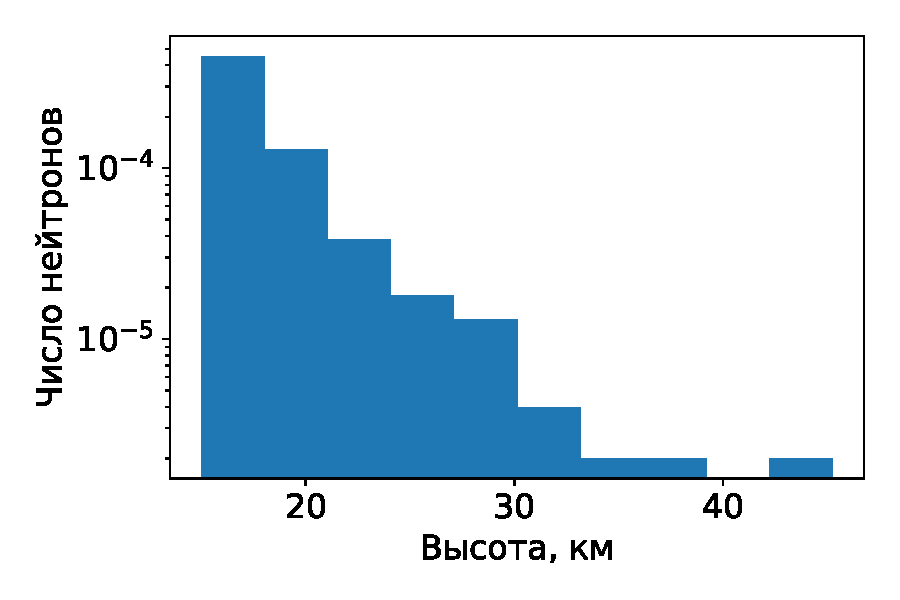
\includegraphics[width=\linewidth]{thunderstorm/neutron/air_z_15MeV.pdf} \\ а)}
        \end{minipage}
        \hfill
        \begin{minipage}[h]{0.49\linewidth}
            \center{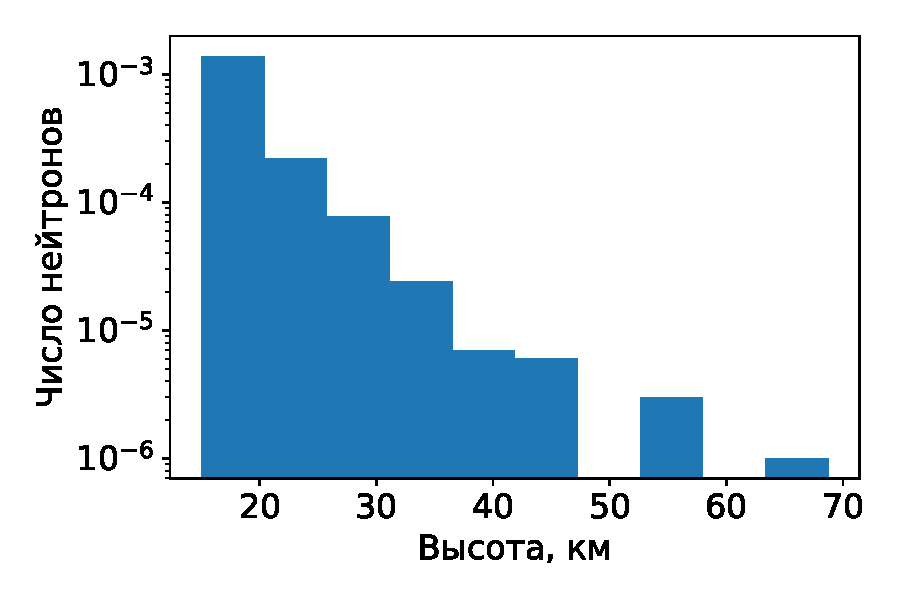
\includegraphics[width=\linewidth]{thunderstorm/neutron/air_z_100MeV.pdf}   \\ б)}
        \end{minipage}
        \caption{Распределение рождения нейтронов по высоте для фотонов с начальной энергией а) 15 МэВ б) 100 МэВ. Нормировано на одну первичную частицу.}
    \end{center}
    \label{fig:storm:neutron_z}
\end{figure}

По результатам моделирования для гамма-квантов с начальной энергией 100 МэВ получено что рождается примерно 1,7 на тысячу гамма-квантов с энергией 100 МэВ. Примерно половина нейтронов имеет энергию до 10 МэВ, вторая часть имеет медленно спадающий спектр в диапазоне от 10 до 70 МэВ. Разброс при рождении в атмосфере достаточно мал, порядка 85 \% нейтронов рождаются в стволе пучка гамма-квантов. Направление импульса рожденных нейтронов имеет достаточно широкий разброс, не позволяющий говорить о наличии выделенного направления движения. График~\ref{fig:storm:neutron_z}а показывает распределение точек рождение нейтронов по высоте. Как мы видим нейтроны рождаются на высотах до 70 километров, далее атмосфера становится сильно разреженной для того что бы шанс с рождения нейтрона был достаточно значительный. Можно отметить что в атмосфере взаимодействует только порядка 0.4 \% гамма-квантов, остальные 99.6\% улетают в космос. Также следует учесть то что гамма-кванты могут рождать нейтроны столкнувшись с корпусом космического аппарата (КА) и телом детектора, однако как показало моделирование, даже если считать что все долетевшие до КА частицы взаимодействуют в нем (что вообще говоря невозможно так как требует КА с массо-габаритным характеристикам значительно превосходящими реальные аппараты), то число таких нейтронов будет составлять только 8\% от числа рожденных в атмосфере.

Результаты моделирования для гамма-квантов с начальной энергией 15 МэВ в целом аналогичны, число рожденных нейтронов примерно в три раза меньше чем для 100 МэВ гаммы, они рождаются на высотах до 40 км (график распределения по высоте приведена на рис.~\ref{fig:storm:neutron_z}б). Только 5\% таких гамма-квантов долетает до космоса, и они не выбывают нейтроны с детектора в КА. Вопрос о достижимости детектора на КА рожденными в атмосфере нейтронов  является дискуссионным, простое GEANT4 моделирование показывает достаточно быструю потерю энергии быстрыми нейтронами, однако есть сомнения в точности выбранной модели, также есть работы показывающий что при больших потоков гамма-квантов возможно достижение нейтронами высот больших 400 км (ссылка а чувака). Однако те не менее моделирование показывает что число нейтронов будет не значительным и размещение детектора нейтронов на КА является не целесообразным и гораздо более эффективным является работа по  регистрации непосредственно гамма-квантов которые долетают до КА в больших количествах.
